\section{Protocolo B92}

El protocolo B92 representa un hito fundamental en la criptografía cuántica al demostrar que la seguridad no depende necesariamente de la cantidad de estados utilizados, sino de la propiedad de no ortogonalidad. En particular, este protocolo pone de manifiesto que incluso un conjunto mínimo de dos estados no ortogonales es suficiente para garantizar seguridad frente a un posible espía, debido a la imposibilidad de distinguirlos perfectamente sin introducir perturbaciones detectables (véase, por ejemplo, \cite{gisin2002}).

\subsection{Contexto y propósito}

El protocolo B92 \citep{bennett1992} es una variante simplificada de BB84 \citep{bennett1984} que emplea únicamente dos estados cuánticos no ortogonales \citep{schrodinger1926quantisierung} para codificar la información. Esta reducción disminuye la complejidad conceptual y experimental del sistema, manteniendo la seguridad basada en la imposibilidad de distinguir dichos estados sin introducir perturbaciones.

\subsection{Funcionamiento del protocolo}

El funcionamiento del protocolo B92 se articula en torno al uso de estados no ortogonales, lo que impide que un posible espía pueda obtener información sin alterar el sistema. A partir de este principio, el proceso se desarrolla de forma secuencial en varias fases:

\paragraph{1. Preparación y envío de estados}. Alice genera una secuencia aleatoria de bits clásicos. A continuación, 
codifica cada bit en un estado cuántico:

\begin{itemize}
    \item El bit 0 se codifica como el estado $|0\rangle$ (polarización horizontal).
    \item El bit 1 se codifica como el estado $|{+}\rangle$ (polarización diagonal).
\end{itemize}

Estos estados son no ortogonales, lo que significa que no pueden distinguirse con certeza absoluta mediante una única medición. Alice envía estos estados, uno a uno, a Bob a través de un canal cuántico.

\paragraph{2. Medición de los estados}. Para cada estado recibido, Bob selecciona aleatoriamente una de las dos bases de medida posibles:

\begin{itemize}
    \item La base $\mathcal{B}_0 = \{|0\rangle, |1\rangle\}$.
    \item La base $\mathcal{B}_+ = \{|{+}\rangle, |{-}\rangle\}$.
\end{itemize}

Debido a la no ortogonalidad de los estados enviados por Alicia, en muchos casos 
Bob no puede determinar con certeza qué estado fue enviado. Sin embargo, en 
determinadas situaciones obtiene un resultado concluyente:

\begin{itemize}
    \item Si detecta $|1\rangle$, sabe que Alicia no envió $|0\rangle$, por lo 
    que deduce que el bit era 1.
    \item Si detecta $|{-}\rangle$, sabe que Alicia no envió $|{+}\rangle$, por 
    lo que deduce que el bit era 0.
\end{itemize}

En el resto de los casos, el resultado es ambiguo y se descarta.

\paragraph{3. Filtrado y comparación}

Una vez que Bob ha realizado las mediciones, ambos participantes utilizan un canal clásico autenticado para coordinarse y extraer la información útil del proceso cuántico.  
  
En esta fase, Bob comunica a Alice exclusivamente las posiciones de los fotones para los cuales ha obtenido un resultado concluyente. Es importante destacar que Bob no revela el valor del bit medido, sino únicamente qué posiciones son válidas.  
  
A partir de esta información:  
  
\begin{itemize}  
    \item Alice identifica los bits que corresponden a esas posiciones. 
    \item Ambos descartan todos los eventos no concluyentes.  
\end{itemize}  
  
El resultado de este proceso es una secuencia común de bits denominada \textit{clave en bruto}.  
  
Posteriormente, Alice y Bob realizan una comparación parcial de esta clave y seleccionan aleatoriamente un subconjunto de bits y los comparan públicamente para estimar la tasa de error \textit{QBER} \citep{nielsen2010quantum}.  
  
\begin{itemize}  
    \item Si los valores coinciden en la mayoría de los casos, el canal se considera seguro.  
    \item Si aparece un número significativo de discrepancias, se concluye que ha habido interferencias o un posible ataque, y el protocolo se aborta.  
\end{itemize}  
  
Este procedimiento permite detectar la presencia de un espía, ya que cualquier medición no autorizada introduce perturbaciones en los estados cuánticos, lo que se refleja en un aumento del error en la clave compartida. Como se describe detalladamente en \cite{nielsen2010}, esta detección es posible porque las leyes de la mecánica cuántica impiden obtener información sobre el estado sin modificarlo inevitablemente.

\subsubsection{Codificación de estados}
En la fase inicial, Alice transforma la información binaria clásica en estados cuánticos mediante la preparación de estados con polarizaciones específicas. A diferencia de otros protocolos, el esquema B92 utiliza una base de estados no ortogonales para representar los valores lógicos, tal como se detalla en la Tabla~\ref{tab:codificacion_b92}, vinculando cada bit a un estado de polarización horizontal o diagonal.

\begin{table}[h!]
\label{tab:codificacion_b92}
\centering
\begin{tabular}{ccc}
\hline
\textbf{Bit} & \textbf{Estado} & \textbf{Polarizaci\'{o}n} \\
\hline
0 & $|0\rangle$ & Horizontal (0\textdegree) \\
1 & $|{+}\rangle$ & Diagonal (+45\textdegree) \\
\hline
\end{tabular}
\caption{Codificaci\'{o}n en B92. Fuente: elaboración propia}
\end{table}

\subsubsection{Medición de Bob}

Por su parte, Bob emplea un sistema de detección basado en bases de medida proyectivas diseñadas para identificar el estado ortogonal al que Alice podría haber enviado. Como se resume en la Tabla~\ref{tab:medicion_bob}, esta estrategia permite a Bob obtener un resultado concluyente solo cuando el fotón se detecta en la orientación opuesta al estado codificado, descartando cualquier medición ambigua derivada de la no ortogonalidad. Bob solo acepta resultados concluyentes (detección del estado ortogonal).

\begin{table}[h!]
\label{tab:medicion_bob}
\centering
\begin{tabular}{ccc}
\hline
\textbf{Base} & \textbf{Estados} & \textbf{Detecta} \\
\hline
$\mathcal{B}_0$ & $\{|{0}\rangle, |{1}\rangle\}$ & $\ket{+}$ \\
$\mathcal{B}_+$ & $\{|{+}\rangle, |{-}\rangle\}$ & $\ket{0}$ \\
\hline
\end{tabular}
\caption{Bases de medida. Fuente: elaboración propia.}
\end{table}

\subsubsection{Diagrama de flujo del protocolo}

Con el fin de facilitar la comprensión de la lógica secuencial que rige el protocolo B92, se presenta a continuación un diagrama de flujo  en el que se detallan las etapas críticas de la comunicación. En este esquema se visualiza cómo la seguridad radica en el filtrado de resultados no concluyentes y en la interacción necesaria entre el canal cuántico de envío y el canal clásico de validación.

\begin{figure}[h!]
\centering
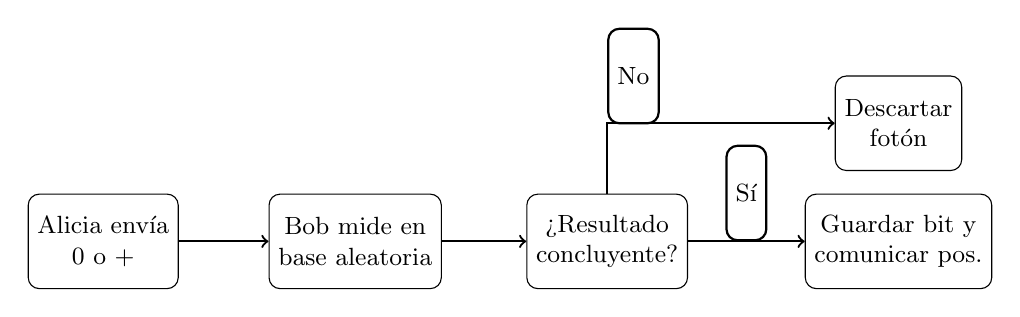
\begin{tikzpicture}[node distance=3.2cm, every node/.style={draw, rectangle, rounded corners, align=center, font=\small, minimum height=1.2cm}]

% Nodos
\node (alice) {Alicia envía\\$\ket{0}$ o $\ket{+}$};
\node (bob) [right of=alice] {Bob mide en\\base aleatoria};
\node (decision) [right of=bob] {¿Resultado\\concluyente?};
\node (yes) [right of=decision, xshift=0.5cm] {Guardar bit y\\comunicar pos.};
\node (no) [above of=yes, node distance=1.5cm] {Descartar\\fotón};

% Flechas
\draw[->, thick] (alice) -- (bob);
\draw[->, thick] (bob) -- (decision);
\draw[->, thick] (decision) -- node[anchor=south] {Sí} (yes);
\draw[->, thick] (decision) |- node[anchor=west, yshift=0.6cm] {No} (no);

\end{tikzpicture}
\caption{Flujo operativo del protocolo B92. Fuente: elaboración propia.}
\label{fig:flujo_b92_horizontal}
\end{figure}

Como se observa en la Figura~\ref{fig:flujo_b92_horizontal}, el flujo resalta el carácter determinista de los bits aceptados por Bob tras la detección de estados ortogonales, reduciendo significativamente la probabilidad de compromiso de la clave compartida antes de las fases finales de post-procesamiento.

\subsection{Ventajas principales}

El protocolo B92 presenta una serie de ventajas que lo sitúan como una alternativa relevante dentro del panorama de los protocolos DV-QKD, ofreciendo un esquema simplificado que mantiene garantías de seguridad incondicional frente a ataques generales \citep{tamaki2003}, destacando principalmente por su extrema simplicidad al requerir únicamente dos estados cuánticos para su funcionamiento. Esta característica constituye su mayor fortaleza, ya que permite una implementación experimental mucho más sencilla que la del protocolo BB84, reduciendo significativamente la complejidad técnica y el diseño del hardware necesario. Asimismo, su seguridad se apoya en un fundamento teórico directo basado en la no ortogonalidad de los estados, permitiendo simplificar la arquitectura del sistema sin comprometer los principios esenciales de la mecánica cuántica que garantizan la confidencialidad en el intercambio de la clave.

%------------------------------------------------------

\subsection{Limitaciones y riesgos}
A pesar de su simplicidad, el protocolo B92 presenta limitaciones que condicionan su uso en entornos reales. Su baja eficiencia en la generación de clave, cercana al 25\% (véase Tabla~\ref{tab:comparativa_b92_bb84}), junto con una mayor sensibilidad al ruido del canal, lo sitúan en desventaja frente a alternativas más robustas, como BB84 con estados señuelo, especialmente en implementaciones de larga distancia o en canales con alta atenuación. En este contexto, \cite{wang2005} mostró que el uso de técnicas de estados señuelo permite reforzar la seguridad de los sistemas prácticos frente a los ataques de tipo \textit{Photon Number Splitting} (PNS), cuya base teórica y peligrosidad en fuentes no ideales fueron formalmente establecidas por \cite{brassard2000pns}. Esta vulnerabilidad es crítica en B92, ya que las imperfecciones en la fuente de los estados pueden permitir a un adversario obtener información de la clave sin introducir el nivel de ruido previsto por el protocolo original.

\begin{table}[h!]
\label{tab:comparativa_b92_bb84}
\centering
\begin{tabular}{ccc}
\hline
\textbf{Característica} & \textbf{B92} & \textbf{BB84} \\
\hline
Estados & 2 & 4 \\
Bases & Implícitas & 2 explícitas \\
Eficiencia & $\sim 25\%$ & $\sim 50\%$ \\
Complejidad & Baja & Media \\
Robustez al ruido & Menor & Mayor \\
Uso práctico & Limitado & Estándar \\
\hline
\end{tabular}
\caption{Comparación entre B92 y BB84. Fuente: elaboración propia.}
\end{table}

%------------------------------------------------------

\subsection{Ejemplo práctico}

A continuación se presenta una ejecución simplificada del protocolo B92 con el objetivo de ilustrar su funcionamiento real. En este ejemplo, Alice genera una secuencia de seis bits aleatorios y los codifica en los estados cuánticos correspondientes, mientras que Bob aplica sus bases de medida de forma aleatoria.


Como se observa en la Tabla~\ref{tab:ejemplo_b92}, únicamente las posiciones 1, 2, 5 y 6 producen resultados concluyentes, descartándose las posiciones 3 y 4 por resultar ambiguas. Esto refleja la eficiencia característica del protocolo, en torno al 66\%, donde solo una fracción de los cúbits enviados contribuye efectivamente a la clave en bruto.

\begin{table}[h!]
\centering
\caption{Ejecución del protocolo B92}
\label{tab:ejemplo_b92}
\begin{tabular}{cccccc}
\hline
\textbf{Pos.} & \textbf{Bit A} & \textbf{Estado} & \textbf{Base B} & \textbf{Resultado} & \textbf{Clave} \\
\hline
1 & 0 & $|0\rangle$ & $\mathcal{B}_+$ & $|{-}\rangle$ & 0 \\
2 & 1 & $|{+}\rangle$ & $\mathcal{B}_0$ & $|1\rangle$ & 1 \\
3 & 1 & $|{+}\rangle$ & $\mathcal{B}_+$ & $|{+}\rangle$ & -- \\
4 & 0 & $|0\rangle$ & $\mathcal{B}_0$ & $|0\rangle$ & -- \\
5 & 1 & $|{+}\rangle$ & $\mathcal{B}_0$ & $|1\rangle$ & 1 \\
6 & 0 & $|0\rangle$ & $\mathcal{B}_+$ & $|{-}\rangle$ & 0 \\
\hline
\end{tabular}
\end{table}

\[
\text{Clave final: } 0, 1, 1, 0
\]

\subsubsection{Presencia de un espía}

Si Eve intercepta los fotones, introduce errores en la clave. Al comparar una muestra, Alice y Bob detectan un aumento del QBER, lo que permite identificar el ataque y abortar la comunicación.

\begin{table}[h!]
\centering
\caption{Resumen técnico del protocolo B92}
\begin{tabular}{lp{8cm}}
\hline
\textbf{Parámetro} & \textbf{Descripción y Valor} \\
\hline
\textbf{Familia} & DV-QKD (Variable Discreta). \\
\textbf{Nº de estados} & 2 estados no ortogonales ($\ket{0}$ y $\ket{+}$). \\
\textbf{Nº de bases} & 2 bases de medida ($\mathcal{B}_0$ y $\mathcal{B}_+$). \\
\textbf{Eficiencia teórica} & 25\% (solo 1 de cada 4 fotones genera clave). \\
\textbf{Seguridad} & Basada en el principio de no clonación y discriminación de estados no ortogonales. \\
\textbf{Punto fuerte} & Extrema simplicidad en la preparación de estados. \\
\textbf{Punto débil} & Alta sensibilidad al ruido y baja tasa de generación de clave (\textit{key rate}). \\
\textbf{Estado actual} & Relevante teóricamente; uso práctico limitado frente a variantes de BB84 con estados señuelo. \\
\hline
\end{tabular}
\end{table}